\chapter{Introduction}
\label{sec:intro}

%\textbf{Thesis Statement}: Malware, and especially Info Theft Malware, on Mobile Operating Systems, especially Android, is better understood when not just analyzing the capabilities of an application, but the expectations the user has as to how it utilizes those capabilities as well.\\
\textbf{Thesis Statement}: Android Malware detection is complemented by not just analyzing the capabilities of an app, but the context and use as well.\\
\textbf{Thesis Statement}: In order to detect Android Malware, the user must understand what is going on behind the scenes of the app. The capabilities of an app are important, but the context and use of these capabilities are as well.\\
\textbf{Thesis Statement}: The transparency of app behavior, letting the user understand the context and use of capabilities, is crucial to understand Android Malware\\


The rise of smartphones in the last decade years has been nothing short of meteoric. Since the launch of the Apple iPhone in 2007, there are now almost 1 Billion smartphone users in the world\citep{kpcbinternetreport2012}. These new devices marked an unprecedented shift in our relationship with computers, becoming the center point for many personal endeavors, and superseding almost all previous computing devices from cell phones, to cameras, to GPS devices, and to most uses of a desktop PC\citep{hua2012introduction}. Indeed, smartphones continue to become the focal point of almost all personal computing, and consequently the operating systems they run become more important and powerful.

\begin{figure}[h]
\begin{center}
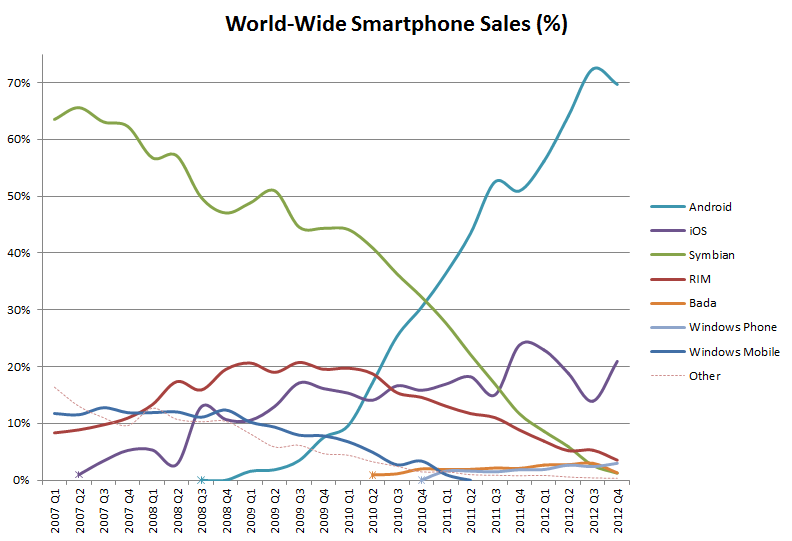
\includegraphics[width=0.8\columnwidth]{figs/World_Wide_Smartphone_Sales_Share}
\caption{Worldwide Market Share of various mobile OSs - from \citep{wikimobileshare} and \citep{gartnerq42012}}
\label{fig:mobileshares}
\end{center}
\end{figure}


Mobile OSs, like the PC operating systems of the 1990s, have a few major players that wield the most influence, as seen in Figure \ref{fig:mobileshares}. The two largest operating systems in the mobile area are Android and iOS. Apple's iOS, made exclusively for the Apple iPhone and iPad, as of the end of 2012, runs on over 20\%\citep{gartnerq42012} of all smartphones globally. Google's Android, released as an open source OS, has many different hardware manufacturers, Samsung, LG, HTC, Motorola, and many more. It currently runs the majority of smartphones globally, with 70\%\citep{gartnerq42012}  marketshare. Some of the less popular, but still significant mobile operating systems are Windows Phone, with 3\%, and Blackberry, with 3.5\%\citep{gartnerq42012} . 

\section{iOS}
Apple released the iPhone in 2007. ``Entry into mobile phones might have been a risky move for Apple. The industry was dominated by Nokia, Motorola, and Samsung, with roughly 60\% market share.''\citep{yoffie2010apple}. However, ``the Apple iPhone was a huge success. Considered by Time magazine the invention of the year 2007 (Invention of the year: the iPhone, Time 2007), it completely changed the mobile phones industry dynamics.''\citep{reis2012leadership}. Apple's iPhone and iOS were novel thanks to it's touch friendly and intuitive OS, and their digital distribution platform, the App Store\citep{yoffie2010apple}, and in 2012, Apple sold over 130 Million iOS devices\citep{gartnerq42012}.

\begin{figure}[h]
\begin{center}
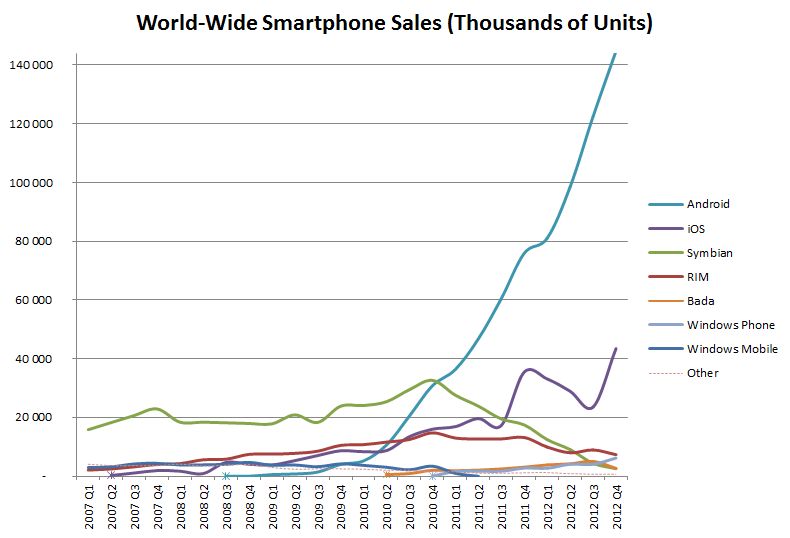
\includegraphics[width=0.8\columnwidth]{figs/World_Wide_Smartphone_Sales}
\caption{Worldwide Sales of various mobile OSs - from \citep{wikimobilesales} and \citep{gartnerq42012}}
\label{fig:mobilesales}
\end{center}
\end{figure}


\section{Android}
Started in 2003 by Andy Rubin and Android, Inc (previously the makers of the T-Mobile Sidekick), Android was acquired by Google Inc in 2005\citep{businessweek2005}. ``Android was built from the ground-up to enable developers to create compelling mobile applications that take full advantage of all a handset has to offer. It was built to be truly open. For example, an application can call upon any of the phone’s core functionality such as making calls, sending text messages, or using the camera, allowing developers to create richer and more cohesive experiences for users''\citep{ohaandroidoverview}. Since it's initial release in 2007\citep{oharelease2007}, Android has skyrocketed to the most used mobile OS in the world, with over 70\% marketshare, and 144 Million Android devices being sold in Q4 of 2012 alone\citep{gartnerq42012} - more than Apple had the entire year, as seen in Figure \ref{fig:mobilesales}.



\section{Goals of Mobile OSs}
For all these mobile OSs, they share many common goals and challenges. The diversity of hardware that smartphones were designed to replace, along other constraints and features, requires a mobile OS that's designed from the ground up to deal with many different challenges than the typical PC OS. Some of the main design challenges for a mobile OS are: 
\begin{smitemize}

\item Small memory footprint, battery conscious, and other resource constrictions

\item Access to a wide variety of personally identifiable information (PII)

\item Access a wide array of hardware

\end{smitemize}
In order to effectively enforce rules on battery consumption, low-latency UI, and personally identifiable information, a new security model was created, centered around the concept of the ``App''. 

%This security model has dramatically changed the nature of mobile software, and in turn, mobile malware. By forcing malware to fit inside of this security sandbox, malware authors must choose to either break out of the box, or work inside of it. This constriction has blurred the definition of mobile malware, and ultimately has profound implications for the user of the mobile device. We will examine these implications, and propose new tools and methods to help understand the nuances of modern malware, as well as provide a framework of tools to detect them.

